\documentclass{beamer}
\usepackage[style=alphabetic]{biblatex}
\addbibresource{bibliography.bib}

\usetheme{CambridgeUS}
\logo{
\includegraphics[width=1.3cm]{images/logo}}

\title[Hate speech at meta]{Hate speech at meta\\ \footnotesize{How
    contrasting hate speech online is a core part of Meta social
    business model}}

\author{Luca Zaninotto}
\institute{Univerità di Padova}
\date{\today}

\begin{document}

\begin{frame}
  \titlepage
\end{frame}

\begin{frame}{Overview}
  \tableofcontents
\end{frame}

\section{Meta business model}
\begin{frame}{Core applications}
  \begin{figure}
    
\includegraphics[width=.4\textwidth]{images/fb.png}
    \hfill
    
\includegraphics[width=.4\textwidth]{images/ig.png}
  \end{figure}
\end{frame}

\begin{frame}{Meta social platforms business model}
  \begin{figure}
    \centering
    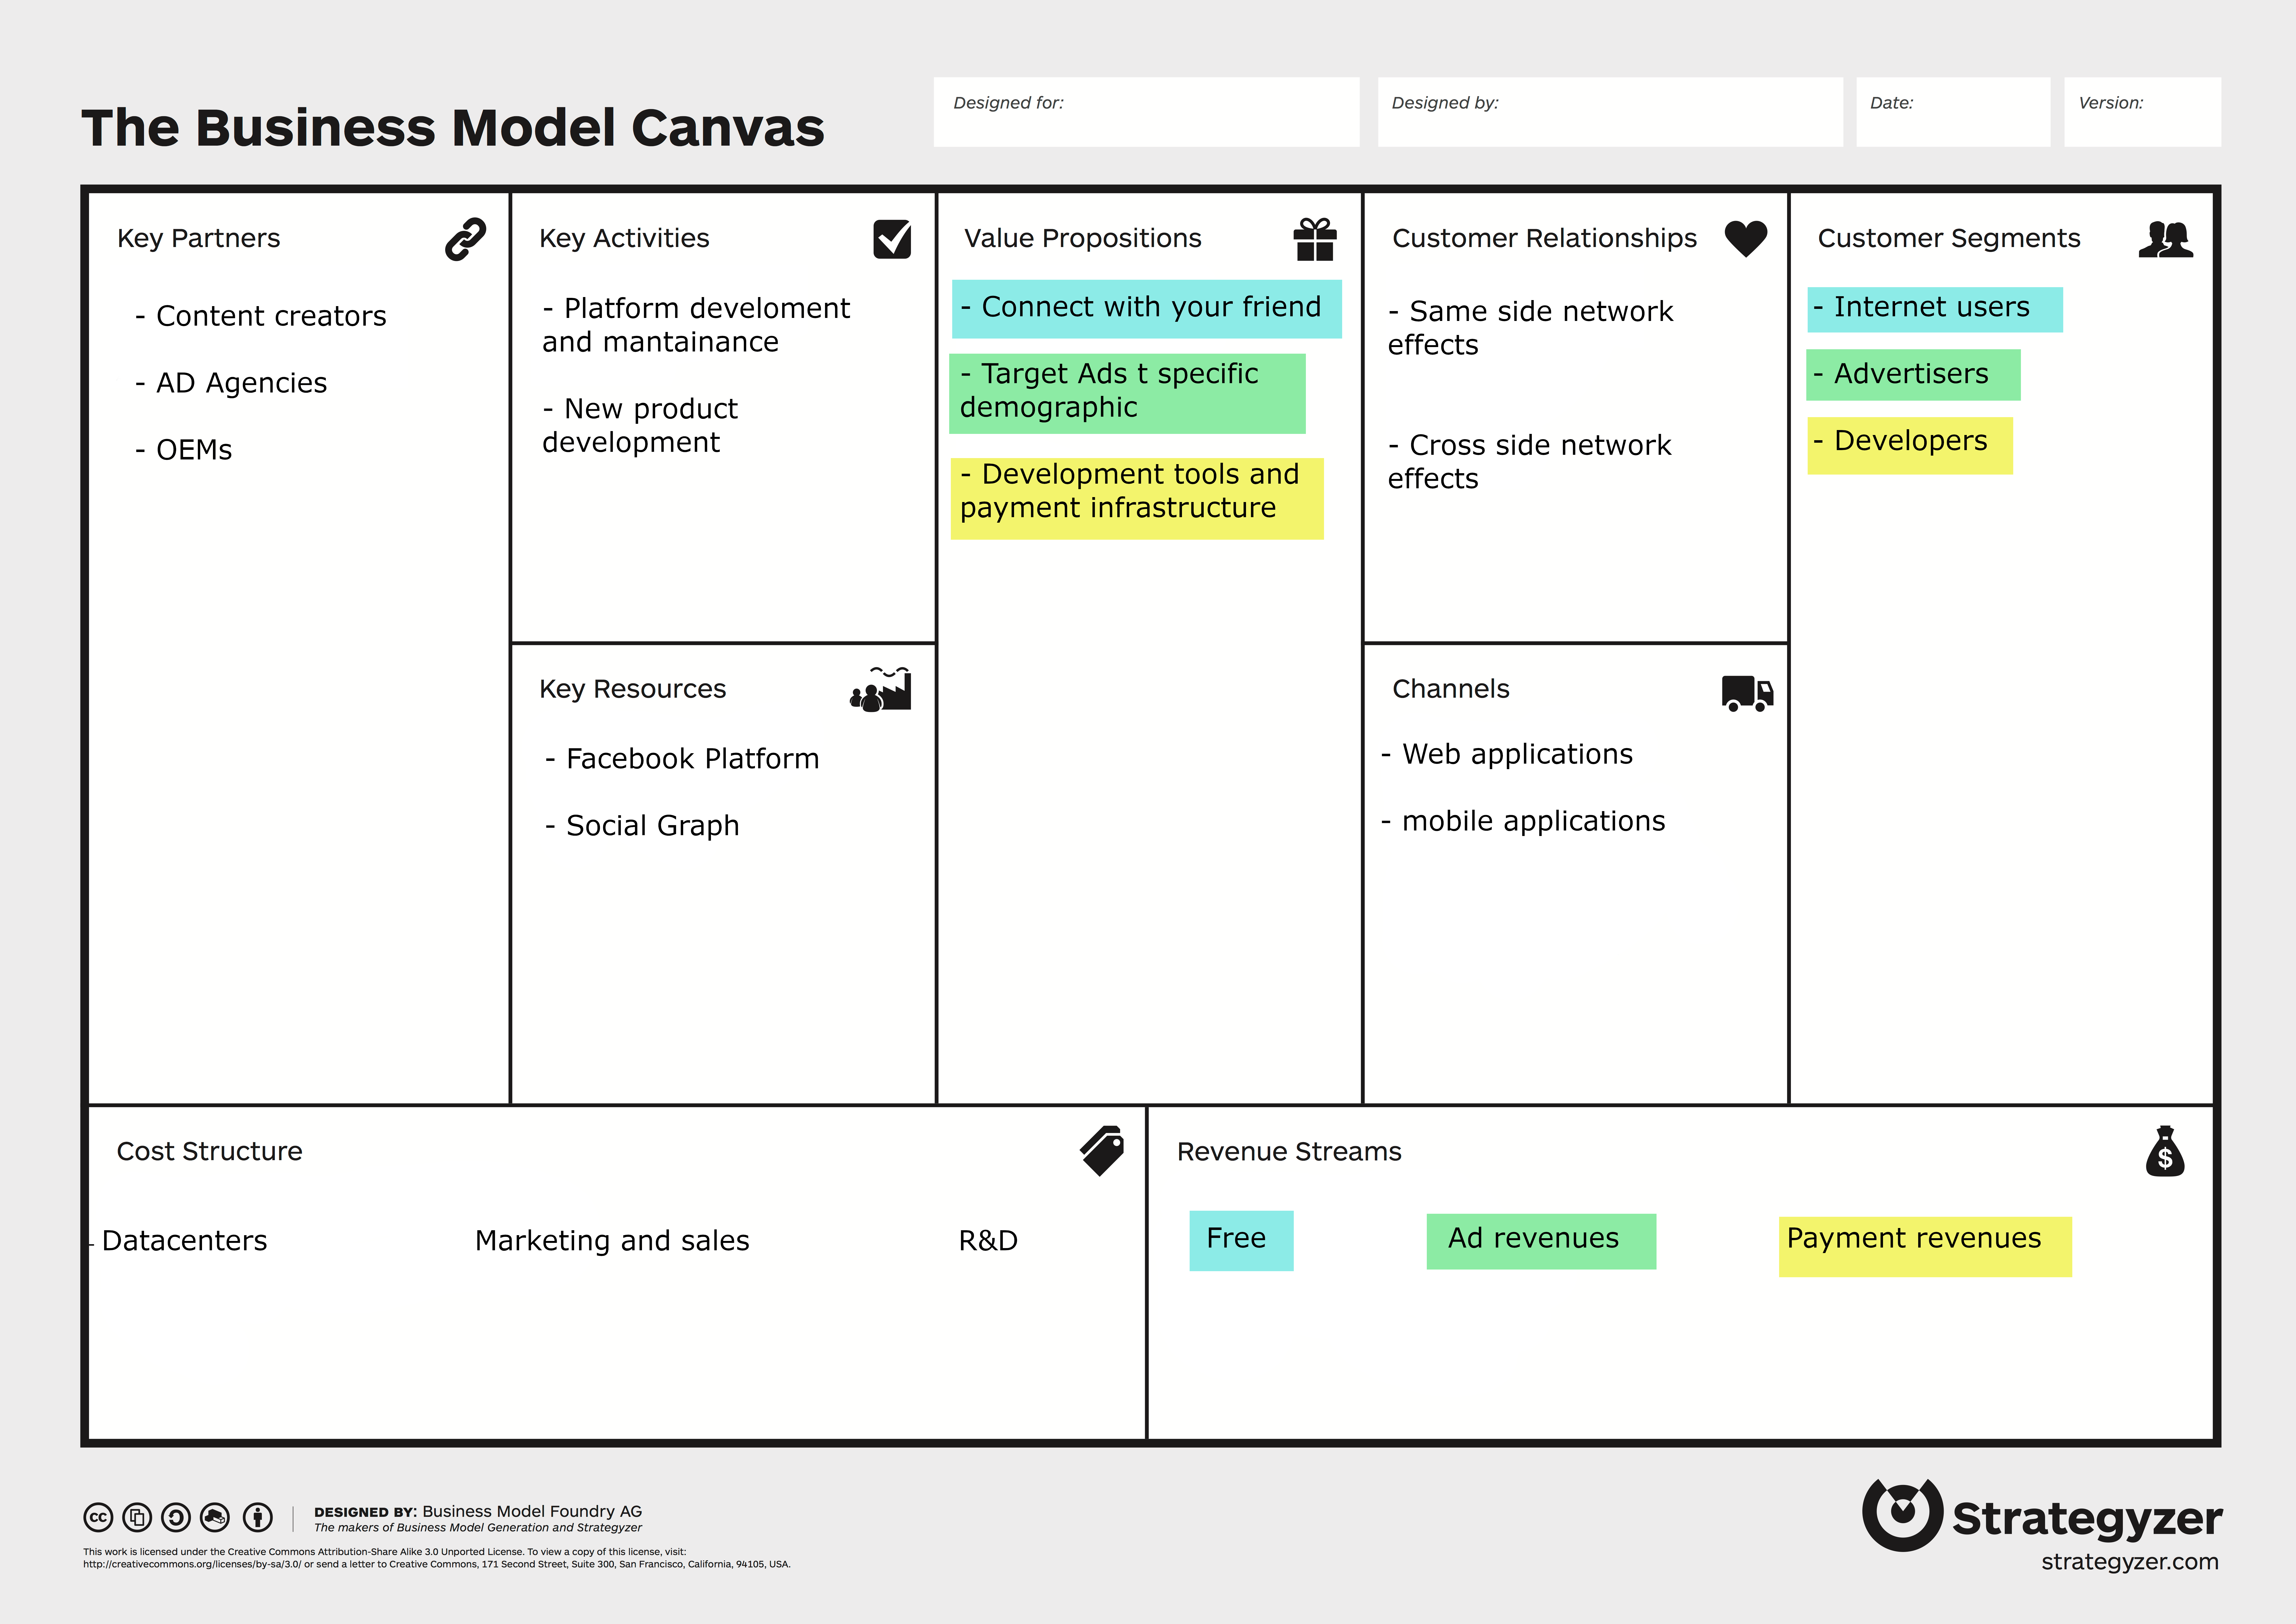
\includegraphics[width=.8\textwidth]{images/fbcanvas}
  \end{figure}
\end{frame}

\begin{frame}{Key factors}
  \begin{itemize}
  \item The relationship with customers is a key component of Meta
    business model.
  \item Factors that create a sense of distrust between the company
    and the customers puts in real danger the whole system.
  \end{itemize}
\end{frame}

\begin{frame}{Hate speech}
  \begin{itemize}
  \item Huge amount of users leads to different subgroups, one that
    disagrees with another in come ways
  \item Misleading content that promotes violence \pause
  \item Users dont want to 
  \end{itemize}
\end{frame}

\section{Innovative AI}
\begin{frame}{A continuous journey}
  \begin{itemize}
  \item Meta started in 2016 to use AI to detect harmful content
    online
  \item New and new technologies started to emerge in order to
    contrast HS since then.
  \item One of the main problems was the evolution of language
  \end{itemize}
\end{frame}

\begin{frame}{New model}
  \begin{figure}
    \centering
    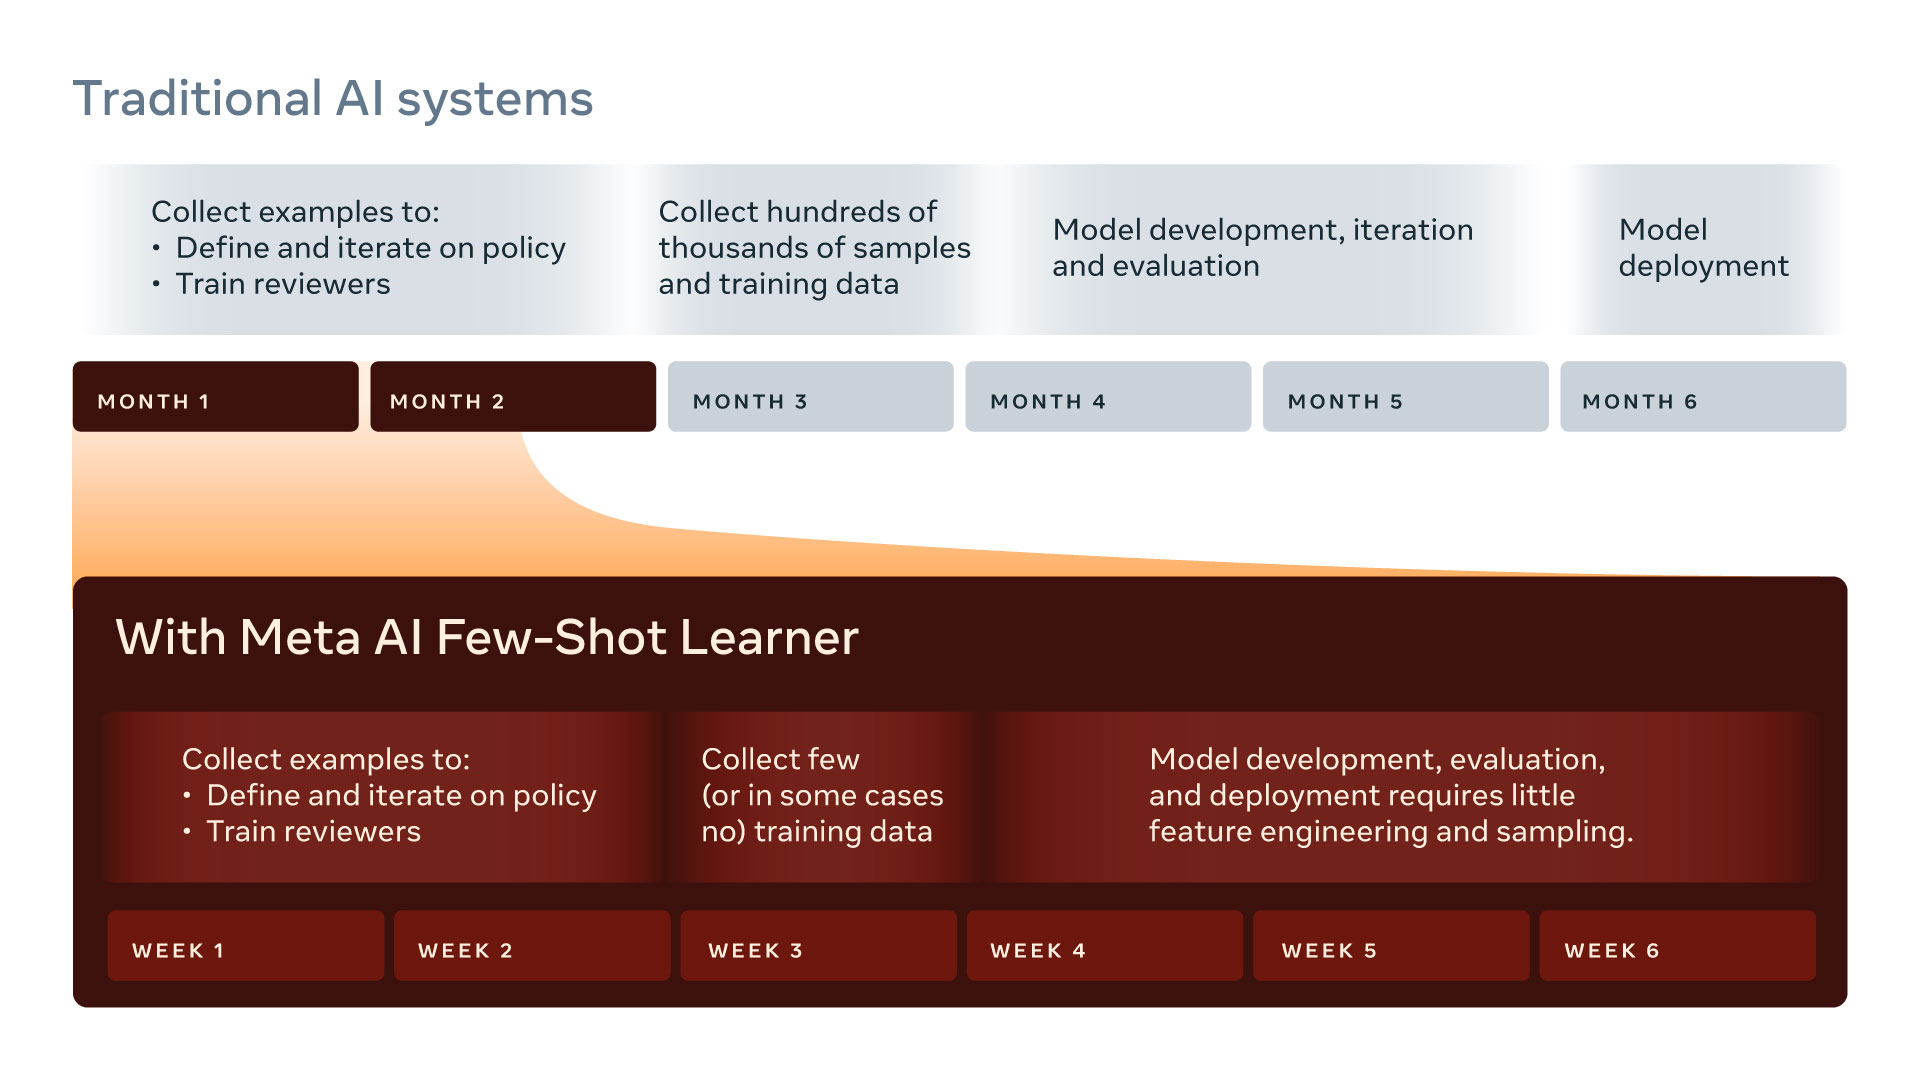
\includegraphics[width=.8\textwidth]{images/fsl_timeline}
    \caption{source: \cite{site:AIart2}}
  \end{figure}
\end{frame}

\begin{frame}{Today's technology}
  \begin{figure}
    \centering
    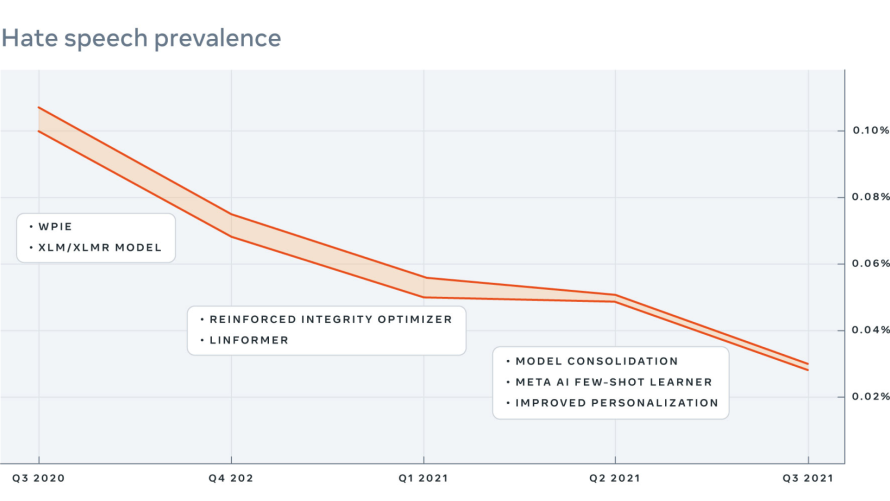
\includegraphics[width=.8\textwidth]{images/fsl_chart}
    \caption{source: \cite{site:AIart}}
  \end{figure}
\end{frame}

\begin{frame}
  \begin{enumerate}
  \item What kind of innovation is this?
  \item How does this innovation affect Meta business model?
  \end{enumerate}
\end{frame}

\section{New value in the business model}
\begin{frame}{Business model innovation}
  \begin{figure}
    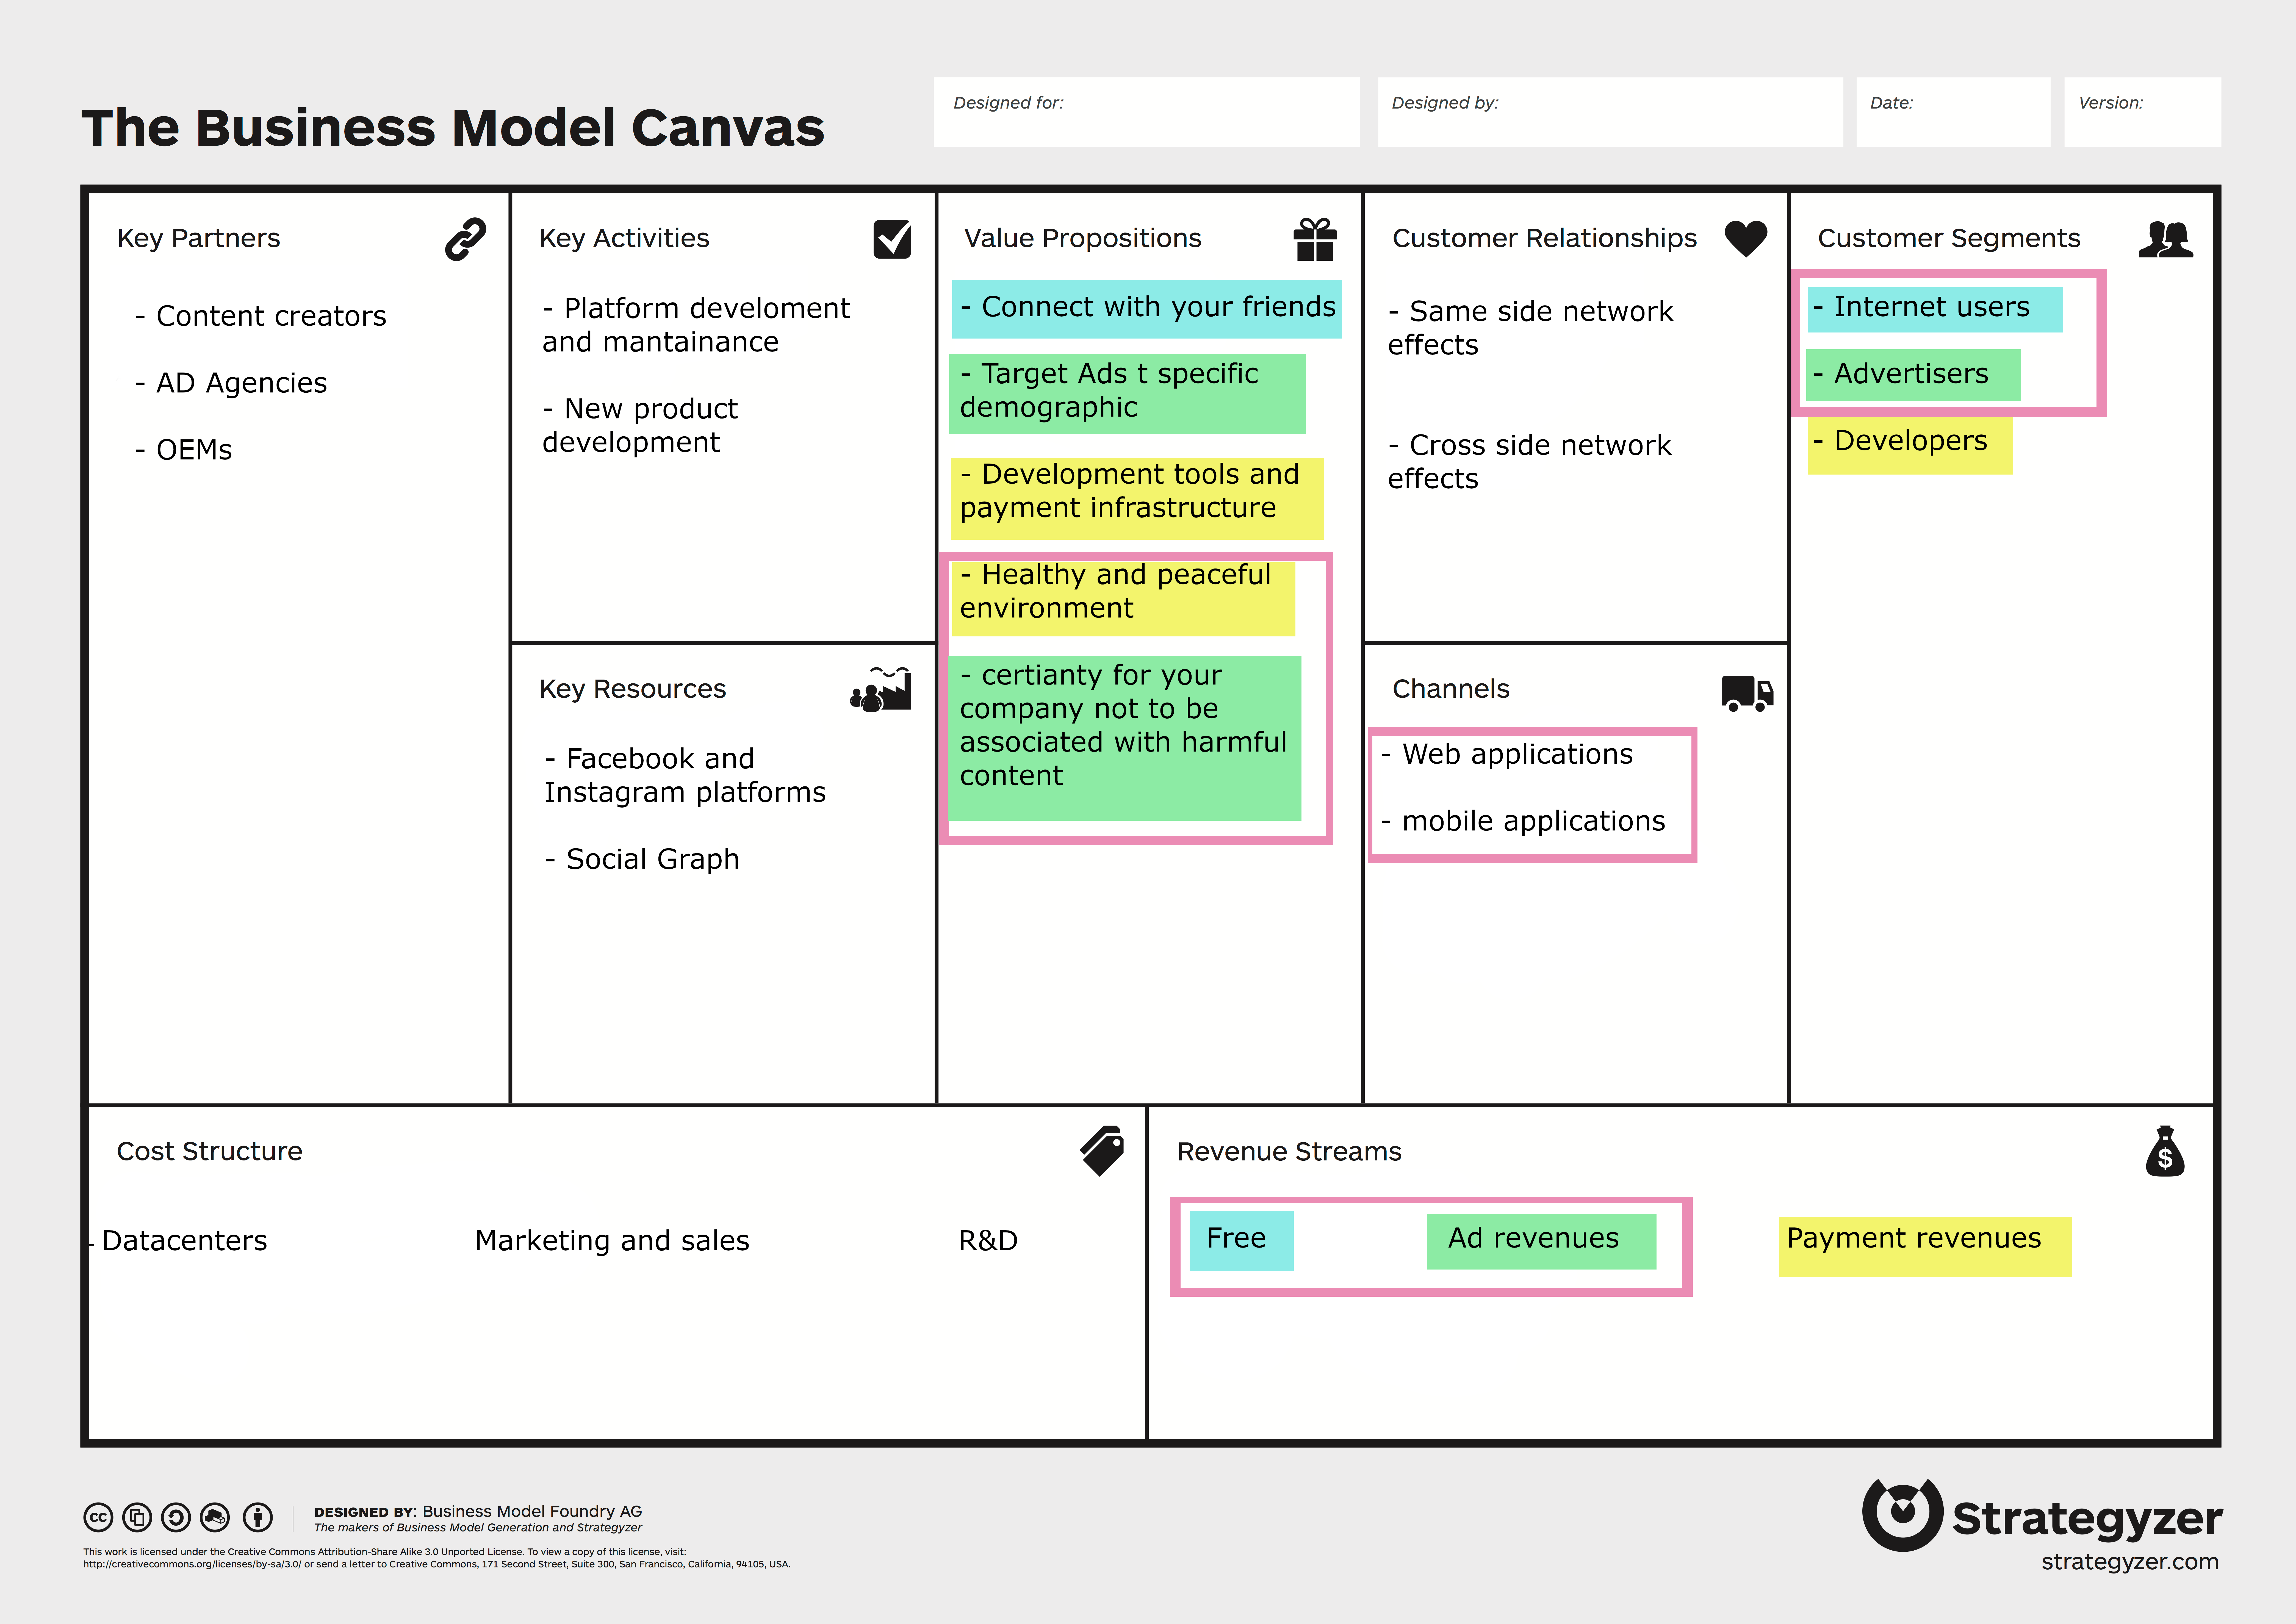
\includegraphics[width=.8\textwidth]{images/newcanvas.png}
  \end{figure}
\end{frame}

\section*{References}
\begin{frame}{References}
  \printbibliography
\end{frame}

\end{document}